\section{Eigenkapital}

\textbf{Risiko der Eigenkapitalgeber}: Eigenkapital wird nachrangig bedient (z.B. bei Insolvenz) $\rightarrow$ EK-Kosten $>$ FK-Kosten\\

\textbf{Venture Capital}: Frühphasenfinanzierung für Unternehmen. \textbf{Quellen}:
\begin{itemize}
	\item Business Angels
	\item Venture Capital Gesellschaften
	\item Öffentlich geförderte, nicht renditeorientierte Beteiligungsgesellschaften
\end{itemize}

\textbf{VC-Finanzierung ist geprägt durch}:
\begin{itemize}
	\item Zurverfügungstellung von haftendem Eigenkapital
	\item Mehrheitsbeteiligung
	\item Zeitliche Befristung der Finanzierung 
	\item Strategische Partnerschaft, bei der der Venture Capitalist das Management mit Beratungsleistungen unterstützt
	\item Strukturierung der Vertragsbeziehung
\end{itemize}
\bigskip
\textbf{Börsengang (Initial Public Offering)}: Aktien eines noch nicht börsennotierten Unternehmens werden zum Kauf angeboten und nach diesem Verkaufsvorgang an der Börse gehandelt

$\rightarrow$ Dient der Eigenkapitalbeschaffung und dem Austritt von Investoren

\textbf{Herkunft der angebotenen Aktien}:
\begin{itemize}
	\item Verkauf durch Altaktionäre (keine Kapitalerhöhung)
	\item Verkauf von Aktien aus einer Kapitalerhöhung
	\item \textbf{Mixed Offering}: Kombination aus beidem
	\item \textbf{Equity-Carve-Out}: Unternehmensteile werden durch Ausgliederung, Abspaltung und Verkauf an die Börse gebracht
\end{itemize}
\bigskip
\textbf{Beteiligte Parteien am Börsengang}:
\begin{itemize}
	\item Unternehmen (Management, Alteigentümer)
	\item Begleitung durch mindestens eine Investment Bank (Underwriter)
	\item Häufig: Emissionskonsortium, Beratungsunternehmen
\end{itemize}
\pagebreak
\textbf{Bookbuilding-Verfahren}:
\begin{itemize}
	\item Veröffentlichung einer Preisspanne, i.d.R. so, dass Überzeichnung resultiert
	\item Erteilung Zeichnungsaufträge von Investoren
	\item Emissionsbank legt endgültigen Preis fest
\end{itemize}
\bigskip
\textbf{Nutzen eines Börsengangs}:
\begin{itemize}
	\item Überwindung von Finanzierungsrestriktionen
	\item Niedrigere Finanzierungskosten
	\item Diversifikation
	\item Kontrolltransfer
	\item Ausnutzung von Fehlbewertungen
\end{itemize}

\textbf{Kosten des Börsengangs}:
\begin{itemize}
	\item \textbf{Direkte Kosten}: Gebühren der Emissionsbanken, weitere Gebühren und Beratungshonorare
	\item \textbf{Indirekte Kosten}: Zeit des Managements, Underpricing, Overallotment Option, Negative Aktienkursreaktion bei Seasoned Offerings
\end{itemize}
\bigskip
\textbf{Underpricing}: Emissionspreis der emittierten Aktien ist niedriger als der kurz darauf festgestellte erste Börsenkurs

$\rightarrow$ Messung: Zahl der verkauften Aktien $\cdot$ (Erster Börsenkurs - Emissionspreis)

\textbf{Erklärungsansatz für Underpricing - Winner's Curse}:
\begin{itemize}
	\item Informationsasymmetrie unter den Anlegern: Informierte Investoren kennen den wahren Wert der Aktie, uniformierte nicht
	\item Informierte Anleger beteiligen sich nur an unterbewerteten Emissionen
	\begin{center}
		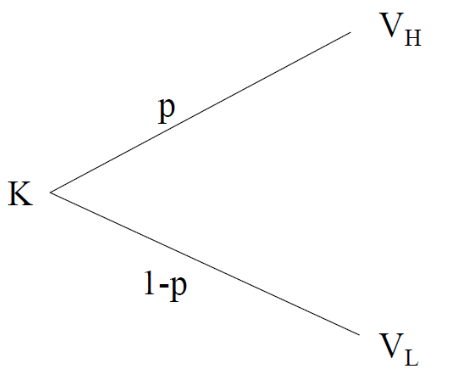
\includegraphics[width=0.25\textwidth]{images/wc.png}
	\end{center}
	\item $V_H$: Hoher Wert der Aktie, $V_L$: Niedriger Wert der Aktie, $K$: Emissionspreis
	\item $p$: Wahrscheinlichkeit für $V_H$, $1-p$: Wahrscheinlichkeit für $V_L$
	\item Unbedingter Erwartungswert: $\overline{V}=pV_H+(1-p)V_L$
\end{itemize}

Sei weiter:
\begin{itemize}
	\item $z$ = Anzahl zu platzierender Aktien
	\item $N$ = Anzahl der potentiellen Zeichner der Aktie
	\item $\pi$ = Anteil informierter Anleger mit $\pi\cdot N<Z$ (weniger informierte Anleger als Aktien) und $(1-\pi)\cdot N>Z$ (mehr uninformierte Anleger als Aktien)
\end{itemize}

Nun gilt:
\begin{center}
	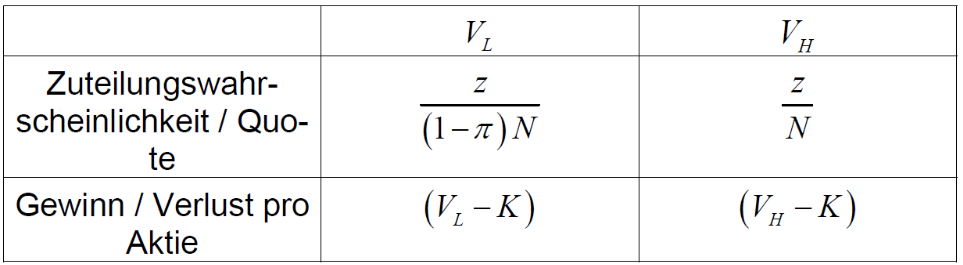
\includegraphics[width=0.55\textwidth]{images/wc-2.png}
\end{center} 

Damit uninformierte Anleger mitzeichnen und die Aktie gleichzeitig nicht zu günstig ist, muss gelten:
$$E(G_u)=p\frac{z}{N}(V_H-K)+(1-p)\frac{z}{(1-\pi)N}(V_L-K)=0$$
wobei $E(G_u)$ der erwartete Gewinn für die uninformierten Anleger ist.

Aufgelöst nach $K$ ergibt sich: 
$$K=\overline{V}-\frac{p(1-p)\pi}{1-p\pi}(V_H-V_L)<\overline{V}$$
also kommt es im Gleichgewicht zum Underpricing

\textbf{Erklärungsansatz für Underpricing - Aktionärsstruktur}:
\begin{itemize}
	\item Emittent (Management/Altaktionäre) möchte Einfluss auf die Aktionärsstruktur nehmen, die sich beim Börsengang ergibt $\rightarrow$ Underpricing, damit Nachfrage nach den Aktien größer ist als das Angebot
	\item \textbf{Gründe für das Beeinflussen der Aktionärsstruktur}: 
	\begin{itemize}
		\item Streubesitz sichert Einfluss der Manager $\rightarrow$ Manager bevorzugen Streubesitz
		\item Konzentrierte Eigentümerstruktur sichert hohe Kontrollintensität und hohen Unternehmenswert durch Disziplinierung des Managements  $\rightarrow$ Alteigentümer bevorzugen konzentrierte Eigentümerstrukturen
	\end{itemize}
\end{itemize}

\textbf{Erklärungsansatz für Underpricing - Informationen}:
\begin{itemize}
	\item Emissionsbank holt vor der Preisfestsetzung Informationen bei potentiell informierten Anlegern ein
	\item Kein informierter Anleger hätte Anreiz, seine wahre Werteinschätzung offenzulegen, wenn er nachher tatsächlich diesen Preis zahlen müsste $\rightarrow$ Underpricing
\end{itemize}
\bigskip
\textbf{Overallotment Option}: 
\begin{itemize}
	\item Über das \enquote{eigentliche} Emissionsvolumen hinausgehendes Kontingent an Aktien, das die Emissionsbank zusätzlich zum Emissionspreis platzieren kann
	\item Erzielbarer Gewinn ist Bestandteil der Vergütung der Emissionsbank
	\item \textbf{Ziel}: Befriedigung der Nachfrage und Verhindern von Kursschwankungen
\end{itemize}
\bigskip
\textbf{Kapitalerhöhung/Seasoned Offerings}: Kapitalerhöhung durch
\begin{itemize}
	\item Zuführung von Mitteln durch bisherige Eigentümer (Rights offer)
	\item Zuführung von Mitteln durch neue Eigentümer (Cash offer)
	\item Bei Kapitalerhöhung darf der Ausgabepreis der neuen Aktien nicht unter dem Nennwert der Aktien (Anteil mit dem ein Aktionär am Grundkapital einer Aktiengesellschaft beteiligt ist) liegen
	\item Im Durchschnitt negative Marktreaktion auf Ankündigung einer Kapitalerhöhung $\rightarrow$ Mögliche Erklärung: \textbf{Adverse Selektion}
\end{itemize}